\documentclass[12pt]{article}
\usepackage{amsmath,amsfonts}
\usepackage[cm]{fullpage}
\usepackage{graphicx}

\pagenumbering{gobble}

\title{\vspace{-24pt}February Monthly Problem Set}
\author{Due: 12 February 2018}
\date{}


\begin{document} \maketitle \pagestyle{empty}

\begin{enumerate}

\item % Hellenic Math Olympiad 2017 Juniors Q3
% Determine all positive integers $a,b,p$, where $p$ is prime, satisfying the following equation:
% \[ \frac{1}{p} = \frac{1}{a^2} + \frac{1}{b^2}. \]
The given equation is equivalent to
\[
    p(a^2 + b^2) = a^2 b^2.
\]

We note that $p \mid a^2 b^2$, and so either $p \mid a$ or $p \mid
b$. Without loss of generality, let $p \mid a$, so that $a = pk$ for some
natural number $k$. The equation then becomes
\[
    a^2 + b^2 = pk^2 b^2.
\]

We thus have that $b^2 \mid a^2 + b^2$, and so $b^2 \mid a^2$, which
gives us that $b \mid a$. Let $a = mb$ for some natural number $m$. The
equation then becomes
\[
    p(m^2 + 1) b^2 = m^2 b^4,
\]
or equivalently
\[
    p(m^2 + 1) = m^2 b^2.
\]

Since $\gcd(m^2, m^2 + 1) = 1$, this implies that $m^2 \mid p$, and so $m =
1$. This gives us that $a = b$, and so the equation simplifies to
\[
    2p = b^2,
\]
which implies that $a = b = p = 2$. This is indeed a solution since
\[
    \frac{1}{2} = \frac{1}{4} + \frac{1}{4}.
\]

\item % Easy-Med? Germany 2015
%Let $M$ be the midpoint of side $AB$ of $\triangle ABC$ in which $BC>CA$. The perpendicular bisector of $AB$ meets $BC$ in $P$ and $AC$ extended in $Q$. Let $R$ be the foot of the perpendicular from $P$ onto $AC$ and let $S$ be the foot of the perpendicular from $Q$ onto $BC$. Prove that $M$, $R$ and $S$ lie on a straight line.
Since $\angle PRQ = \angle PSQ = 90^\circ$, we have that $P$, $R$, $S$, and $Q$
lie on the circle with diameter $PQ$. Let $O$ be the midpoint of $PQ$, so that
$O$ is the centre of this circle. Since $O$ lies on the perpendicular bisector
of $AB$, we have that $OA = OB$, and so $A$ and $B$ have equal power with
respect to this circle. It follows that $BP \times BS = AR \times AQ$. By
applying Power of a Point in this circle to point $C$, we also have that $CQ
\times CR = CP \times CS$.

By Menelaus's Theorem applied to triangle $\triangle ABC$ and line $MPQ$, we have that
\[
    \frac{AM}{MB} \cdot \frac{BP}{PC} \cdot \frac{CQ}{QA} = -1.
\]

Using that
\[
    \frac{BP}{QA} = \frac{RA}{BS}
\]
and
\[
    \frac{CQ}{PC} = \frac{SC}{CR},
\]
we thus have that
\[
    \frac{AM}{MB} \cdot \frac{RA}{BS} \cdot \frac{SC}{CR} = -1.
\]

Since
\[
    \frac{AM}{MB} = 1
\]
this is equivalent to
\[
    \frac{AM}{MB} \cdot \frac{BS}{SC} \cdot \frac{CR}{RA} = -1,
\]
and so by Menelaus's Theorem, we have that $M$, $R$, and $S$ are collinear.

\begin{center}
    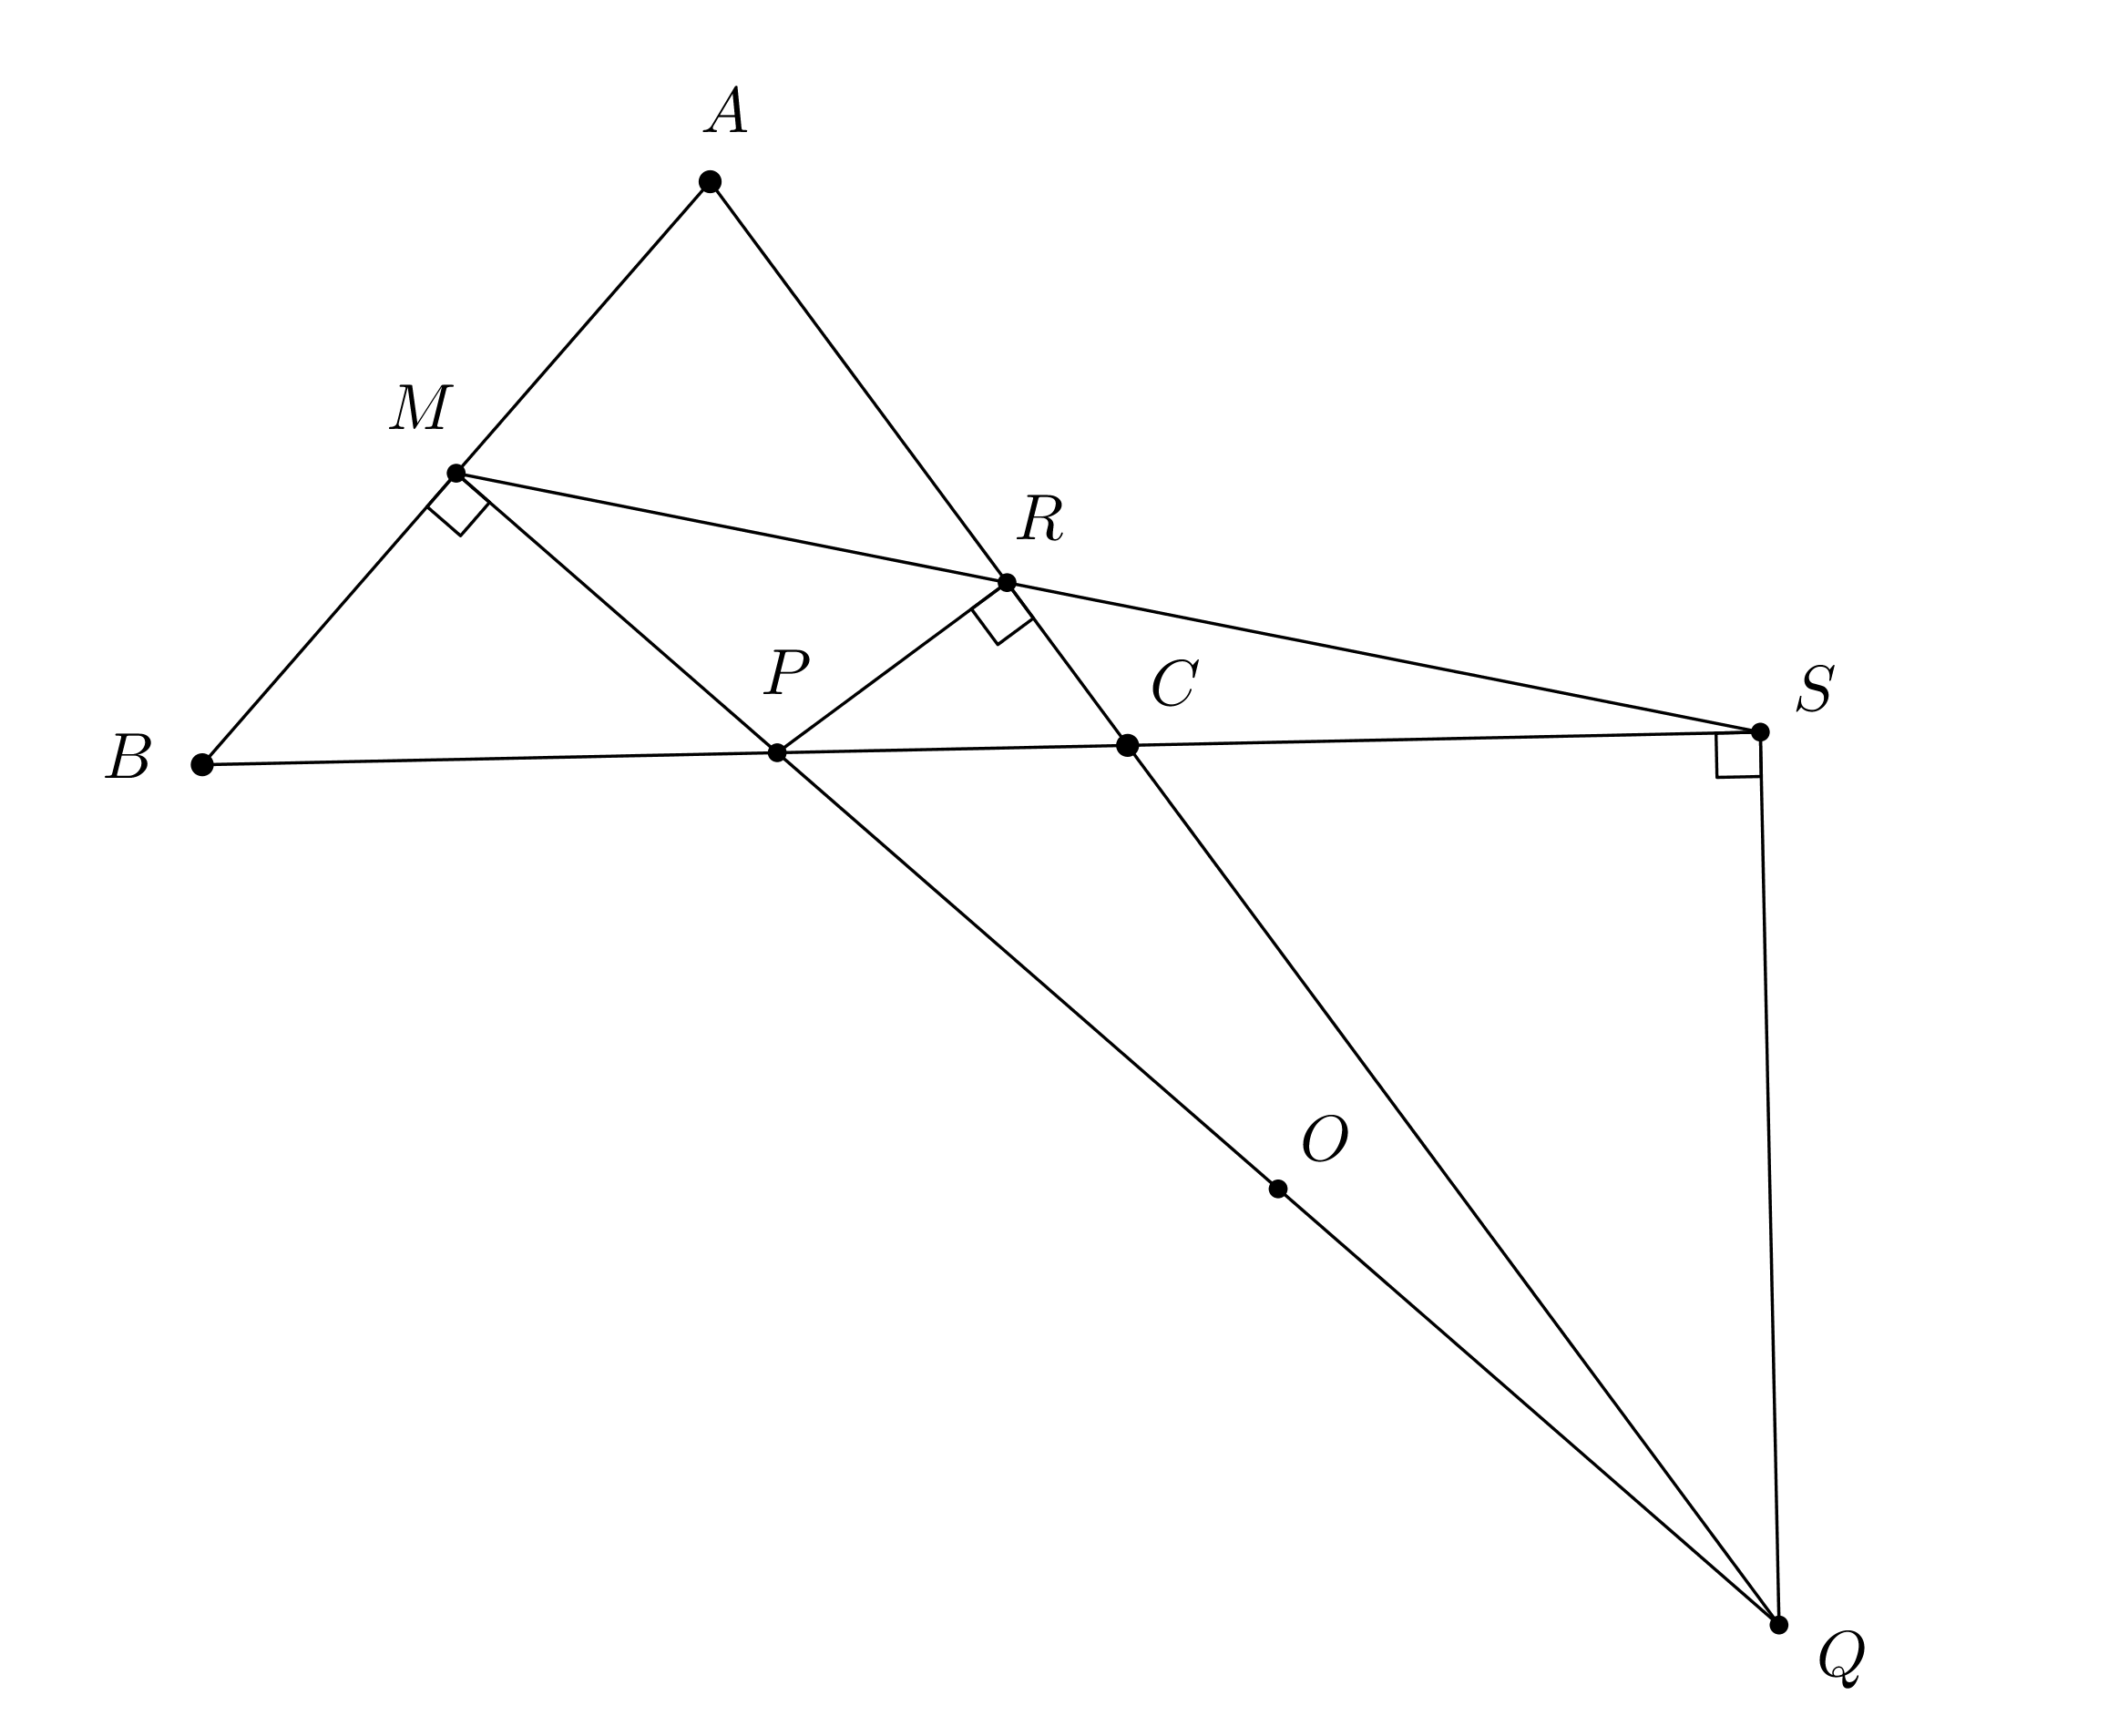
\includegraphics[width=0.8\textwidth]{february_q2.png}
\end{center}


\item % Scry 2, Magic the Gathering
%Consider a deck of $n$ cards with cards numbered from $1$ to $n$. There is one card of each number, but the deck is shuffled, so the cards do not necessarily appear in numerical order. You are allowed to perform the following operation on the deck: You look at the top two cards of the deck, and place one of these two cards on the bottom of the deck, and the other card on top. Show that it is possible, using only this operation some number of times, to sort the deck so that the cards appear in ascending order. 
We will show by induction on $k$ that for $0 \leq k \leq n$, it is possible to
use the allowed move to arrange the deck such that the cards from $1$ to $k$ are
in ascending order at the bottom of the deck. This clearly implies the desired
result.

The claim is vacuously true for $k = 0$. Now suppose that we have the cards from
$1$ to $k$ in ascending order at the botton of the deck. Repeatedly draw two
cards, and place either one at the bottom of the deck, until one of the two
cards that we draw is $(k + 1)$. At this point, place $(k + 1)$ at the top of
the deck, and the other card on the bottom. Now repeatedly draw two cards, and
place $(k + 1)$ at the top of the deck and the other card at the bottom until
the card that we place is the bottom is card number $k$. At this point, we have
$(k + 1)$ at the top of the deck, and the cards from $1$ to $k$ in ascending
order at the bottom of the deck. Now draw two cards, and place $(k + 1)$ at the
bottom of the deck and the other card at the top so that we have the cards from
$1$ to $(k + 1)$ at the bottom of the deck in ascending order as desired.


\item % DB-2012-7
%Determine all triples of real numbers $(x,y,z)$ that simultaneously satisfy the equations:
%\begin{align*}
%	(x^2 - 4x + 7 )(y^2 + 6y + 14) &= 120 \\
%	(y^2 - 6y + 14)(z^2 + 8z + 23) &= 336 \\
%	(z^2 - 8z + 23)(x^2 + 4x + 7 ) &= 96.
%\end{align*}
Note that
\[
    (x^2 - 4x + 7)(x^2 + 4x + 7) = (x^2 + 7)^2 - 16x^2 = x^4 - 2x^2 + 49 = (x^2
    - 1) + 48.
\]

Similarly,
\[
    (y^2 - 6y + 14)(y^2 + 6y + 14) = (y^2 - 4)^2 + 180,
\]
and
\[
    (z^2 - 8z + 23)(z^2 + 8z + 23) = (z^2 - 9)^2 + 448.
\]

Thus multiplying the given equations together, we obtain that
\[
    \left( (x^2 - 1)^2 + 48 \right) \left( (y^2 - 4)^2 + 180 \right) \left( (z^2
    - 9)^2 + 448 \right) = 120 \cdot 336 \cdot 96.
\]

Now the left hand side is greater than or equal to $48 \cdot 180 \cdot 448$,
which conveniently happens to be equal to $120 \cdot 336 \cdot 96$. Since
equality holds, we must have that
\[
    x^2 - 1 = y^2 - 4 = z^2 - 9 = 0.
\]

If $x = 1$, then the equation
\[
    (x^2 - 4x + 7)(y^2 + 6y + 14) = 120
\]
gives us that
\[
    y^2 + 6y + 14 = 30
\]
and so $y = 2$. The equation
\[
    (y^2 - 6y + 14)(z^2 + 8z + 23) = 336
\]
then gives us that
\[
    z^2 + 8z + 23 = 56
\]
and of $z = 3$ and $z = -3$, only $z = 3$ satisfies this equation.

If, on the other hand, $x = -1$, then the equation
\[
    (x^2 - 4x + 7)(y^2 + 6y + 14) = 120
\]
gives us that
\[
    y^2 + 6y + 14 = 10,
\]
and neither $y = 2$ nor $y = -2$ satisfies this equation.

Thus the only solution to the given system of equations is given by $(x, y, z) =
(1, 2, 3)$.



\item % Hard? Dutch IMO Selection 2016
%Determine the number of sets $A = \{a_1,a_2,\ldots, a_{1000}\}$ of positive integers satisfying $a_1 < a_2 < \dotsb < a_{1000} \le 2014$ for which the set
%	\[ S = \{a_i+a_j \mid 1\le i,j\le 1000,\ i+j\in A\} \]
%is a subset of $A$.


\item % SW-2011-4
%Determine the largest integer $C$ such that the inequality \[ (x_1^2+200) +(x_2^2+200) +\dotsb +(x_k^2+200) \geq C \] holds for all positive integers $k$ and all $k$-tuples $(x_1,x_2,\dotsc,x_k)$ of positive integers such that $x_1+x_2+\dotsb+x_k = 100$.
By [instert your favourite inequality here], we know that
\[
    k(x_1^2 + x_2^2 + \dots + x_k^2) \geq (x_1 + x_2 + \dots + x_k)^2 = 10000.
\]

We thus have that
\[
    (x_1^2 + 200) + (x_2^2 + 200) + \dots + (x_k^2 + 200) \geq \frac{10000}{k} +
    200k \geq 2 \sqrt{2 \times 10^6} = 2000 \sqrt{2},
\]
where the last inequality follows from AM-GM. Since $\sqrt{2} > 1.414$, we have
that
\[
    (x_1^2 + 200) + (x_2^2 + 200) + \dots + (x_k^2 + 200) > 2828.
\]

Now $x_i^2$ has the same parity as $x_i$, so we have that
\[
    (x_1^2 + 200) + (x_2^2 + 200) + \cdots + (x_k^2 + 200)  
\]
is an even integer, and hence is at least equal to $2830$. Thus the inequality
holds for $C = 2830$.

To see that $2830$ is the best possible value for $C$, let
\begin{align*}
    x_1 & = x_2 = \dots = x_5 = 14 & \text{and} && x_6 & = x_7 = 15.
\end{align*}
Then 
\[
    x_1 + x_2 + \dots + x_7 = 5 \times 14 + 2 \times 15 = 100,
\]
and
\[
    (x_1^2 + 200) + (x_2^2 + 200) + \dots + (x_7^2 + 200) = 5 \times 14^2 + 2
    \times 15^2 + 7 \times 200 = 2830.
\]


\item % JM-2012-4
%Let $ABC$ be a triangle with circumcentre $O$. Let $\omega_1$ and $\omega_2$ be two circles both with centre $O$ but with different sizes. Let $\omega_1$ intersect $AB$ in $P$ and $Q$ (with $P$ closer to $A$) and $\omega_2$ intersect $AC$ in $R$ and $S$ (with $R$ closer to $A$). Let $RQ$ intersect $BC$ at $K$ and let $PS$ intersect $BC$ at $L$. Prove that $BK = CL$.
We make use of directed line segments.

Since $A$ and $B$ are an equal distance from $O$, they have equal power with
respect to $\omega_1$, and so we have that $AP \times AQ = BP \times BQ$.
Simllarly, since $A$ and $C$ are an equal distance from $O$, they have equal
power with respect to $\omega_2$, and so we have that $AR \times AS = CS \times
CR$.

Applying Menelaus's Theorem to triangle $\triangle ABC$ and line $RQK$, we have
that
\[
    \frac{AQ}{QB} \cdot \frac{BK}{KC} \cdot \frac{CR}{RA} = -1.
\]
Applying Menelaus's Theorem to triangle $\triangle ABC$ and line $PSL$ gives us
that
\[
    \frac{AP}{PB} \cdot \frac{BL}{LC} \cdot \frac{CS}{SA} = -1.
\]
Multiplying these together gives us that
\[
    \frac{AP \times AQ}{PB \times QB} \cdot \frac{BL \times BK}{LC \times KC}
    \cdot \frac{CS \times CR}{SA \times RA} = 1.
\]

But we know that
\[
    \frac{AP \times AQ}{PB \times QB} = \frac{CS \times CR}{SA \times RA} = 1.
\]
and so we have that
\[
    BL \times BK = LC \times KC.
\]

We thus have that
\[
    BK (BC + CL) = LC (KB + BC)
\]
and so
\[
    BK \times BC + BK \times CL = BK \times CL + LC \times BC
\]
giving us that
\[
    BK = LC
\]
as desired.

\begin{center}
    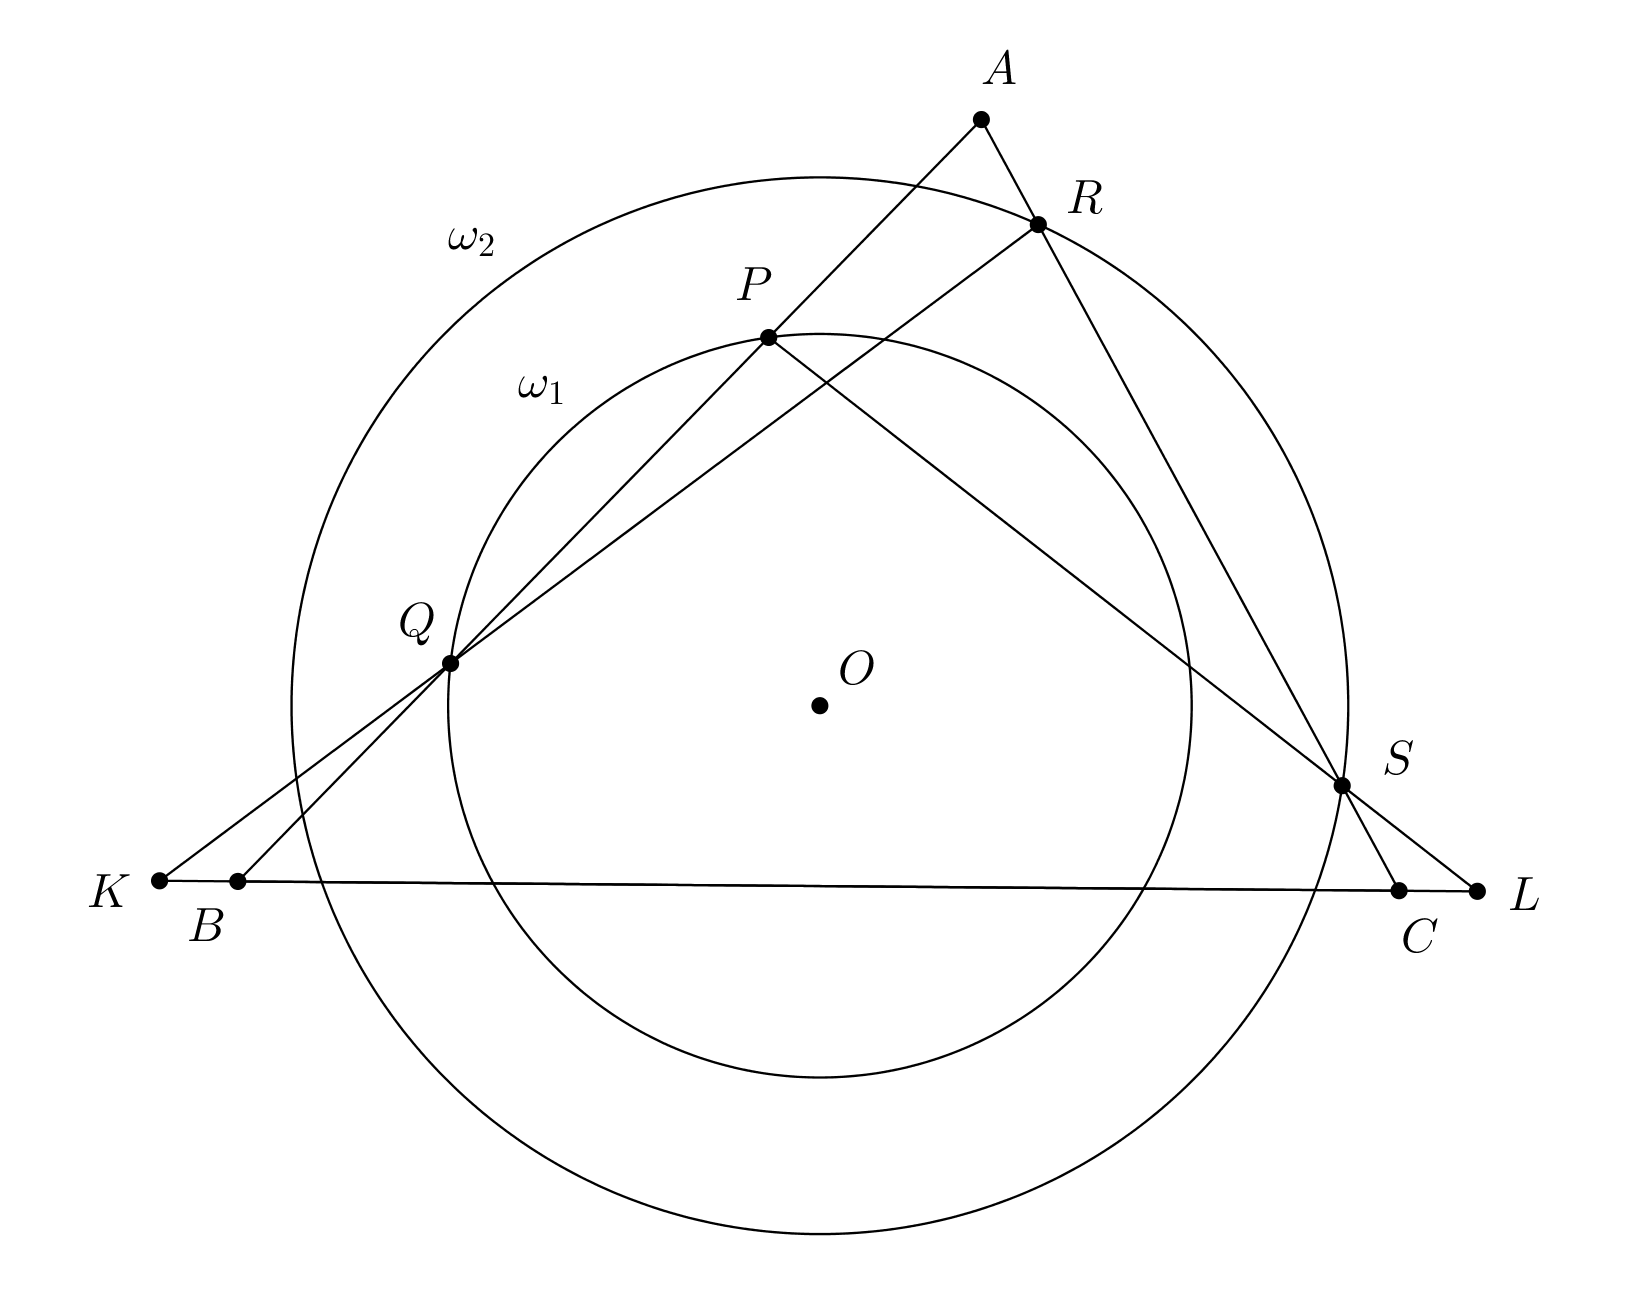
\includegraphics[width=0.8\textwidth]{february_q7.png}
\end{center}

\item % LB-2010-2
%Find all functions $f : \mathbb{Z} \to \mathbb{Z}$ such that for each pair of integers $a$ and $b$, where $a < b$, there exists a prime number $p$ and a nonnegative integer $c$ such that \[ \frac{f(b)-f(a)}{b-a} = p^c. \]
Note that the function $f$ satisfies the condition if and only if the function
$n \mapsto f(n) - f(0)$ does, and so we may assume that $f(0) = 0$.

Also note that exchanging $a$ and $b$ does not alter the value of
\[
    \frac{f(b) - f(a)}{b - a},
\]
and so we may replace the condition that $a < b$ with $a \neq b$.

Let $a = 0$. Then we have that for all $b \neq 0$ that
\[
    \frac{f(b)}{b}
\]
is a power of a prime number.
Let $g$ be the function defined by $f(n) = n \cdot g(n)$ for all $n$, and $g(0)
= 1$. Our previous observation then gives us that $g(n)$ is a power of a prime
for all $n$.

Suppose that there is some $k \neq 0$ such that $g(k) \neq 1$. Let $g(k) = p^c$
where $p$ is a prime number, and let $k = p^s \cdot t$ where $\gcd(p, t) = 1$.

I claim that for all $m > c + s$, that we have that
\[
    g\left( p^m + k \right) = p^c.
\]

Indeed, the condition on $f$ and the definition of $g$ gives us that
\[
    \frac{\left(p^m + k\right) g\left(p^m + k\right) - k \cdot p^c}{p^m} =
    \frac{f\left(p^m + k\right) - f(k)}{\left(p^m + k\right) - k}
\]
is a power of a prime.

Since $p^{c + s}$ divides both $p^m$ and $k \cdot p^c$, this gives us that
\[
    p^{c + s} \mid k \cdot g \left( p^m + k \right) = p^s \cdot t \cdot g \left(
    p^m + k \right),
\]
which implies that
\[
    p^c \mid t \cdot g \left( p^m + k \right),
\]
and since $\gcd(p, t) = 1$, this gives us that
\[
    p^c \mid g \left( p^m + k \right),
\]
and so
\[
    g \left( p^m + k \right) = p^{c + r}
\]
for some non-negative integer $r$. (Since $g$ is always a power of a prime.)

We thus have that
\[
    \frac{p^{c + r} \left( p^m + k \right) - p^{s + c} \cdot t}{p^m}
\]
is a power of a prime.

If $r > 0$, then we note that since $k$ and $p^m$ are both divisible by $p^s$,
we have that
\[
    p^{c + r} \left( p^m + k \right)
\]
is divisible by $p^{s + c + 1}$, and since $\gcd(p, t) = 1$, this implies that
the largest power of $p$ which divides
\[
    p^{c + r} \left( p^m + k \right) - p^{s + c} \cdot t
\]
is exactly $p^{s + c}$. But $p^m > p^{s + c}$, so
\[
    \frac{p^{c + r} \left( p^m + k \right) - p^{s + c} \cdot t}{p^m}
\]
is not an integer, which is a contradiction. Thus we have that $r = 0$, and so
\[
    g \left( p^m + k \right) = p^c.
\]

We thus have that there are arbitrarily large values of $m$ such that $g(m) =
p^c$.

Now consider any $n \neq 0$. For any $m$ such that $g(m) = p^c$, we have that
\[
    n - m \mid f(n) - f(m) = ng(n) - m\cdot p^c,
\]
and so
\[
    m - n \mid ng(n) - m\cdot p^c + (m - n) \cdot p^c = n(g(n) - p^c).
\]

Since this holds for arbitrarily large values of $m$, we must have that
\[
    n(g(n) - p^c) = 0,
\]
and so $g(n) = p^c$. We thus have that $f(n) = n \cdot p^c$ for all $n$, and we
can check that this is a valid solution.

What we have shown is that if there is some $k$ such that $g(k) = p^c \neq 1$,
then $f(n) = n \cdot p^c$ for all $n$. The other possibility is that instead
$g(k) = 1$ for all $k$. This then gives us that $f(n) = n$ for all $n$, and we
can check that this is also a valid solution.

Remembering that we have been dealing with the function $n \mapsto f(n) - f(0)$
rather than $f$, we see that all solutions to the problem are of the form
\[
    f(n) = p^c \cdot n + d
\]
for some prime number $p$, some non-negative integer $c$, and some integer $d$.

\end{enumerate}

\end{document}
